\section{Pruebas satisfactorias}
\begin{frame}

\begin{figure}[!htbp]
    
    \begin{multicols}{2}
     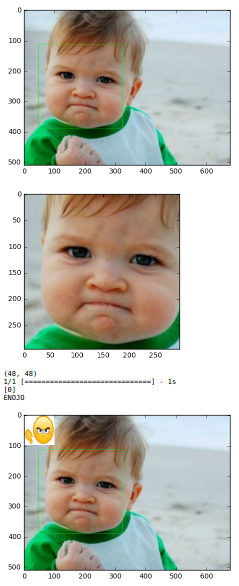
\includegraphics[angle=0,width=48mm]{Imagenes/test1.png}
       \caption{Test 1}
       \label{fig:test1}   
       
       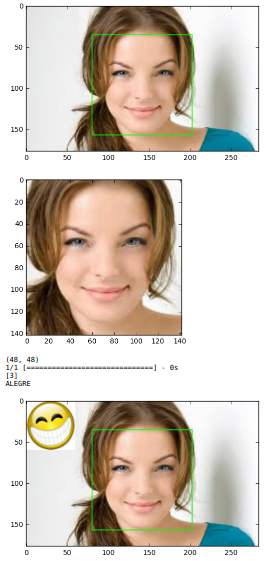
\includegraphics[angle=0,width=55mm]{Imagenes/test2.png}
           \caption{Test 2}
           \label{fig:test2} 
           
    \end{multicols}
        
\end{figure}
\end{frame}


\begin{frame}

\begin{figure}[!htbp]
    
    \begin{multicols}{2}
     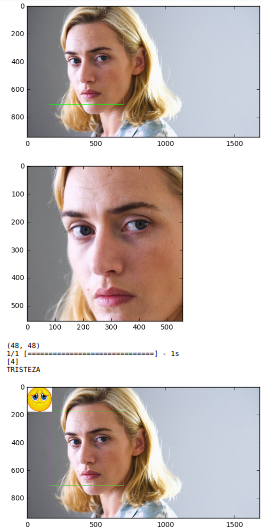
\includegraphics[angle=0,width=50mm]{Imagenes/test3.png}
       \caption{Test 3}
       \label{fig:test3}   
       
       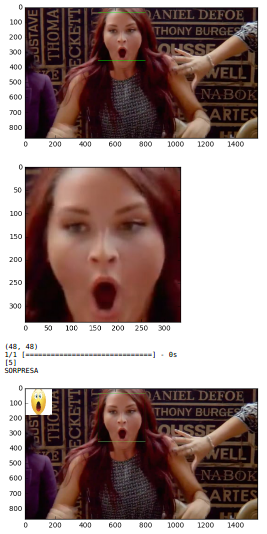
\includegraphics[angle=0,width=50mm]{Imagenes/test4.png}
           \caption{Test 4}
           \label{fig:test4} 

           
            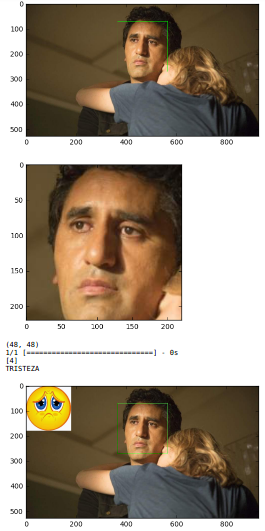
\includegraphics[angle=0,width=50mm]{Imagenes/test5.png}
              \caption{Test 5}
              \label{fig:test5}   
              
              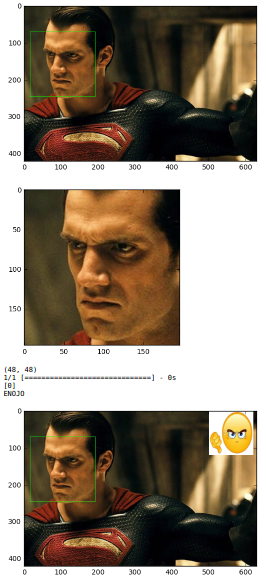
\includegraphics[angle=0,width=50mm]{Imagenes/test6.png}
                  \caption{Test 6}
                  \label{fig:test6}   
                  
                  
    \end{multicols}
        
\end{figure}
\end{frame}


\begin{frame}

\begin{figure}[!htbp]

   \centering
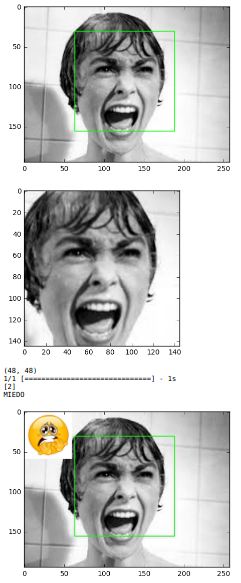
\includegraphics[angle=0,width=50mm]{Imagenes/test7.png}
    \caption{Test 7}
    \label{fig:test7} 

        
\end{figure}
\end{frame}



 
\section{Pruebas Fallidas}
\begin{frame}

\begin{figure}[!htbp]
    
    \begin{multicols}{2}
     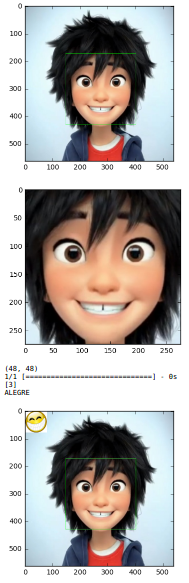
\includegraphics[angle=0,width=48mm]{Imagenes/test8.png}
       \caption{Test 8}
       \label{fig:test8}   
       
       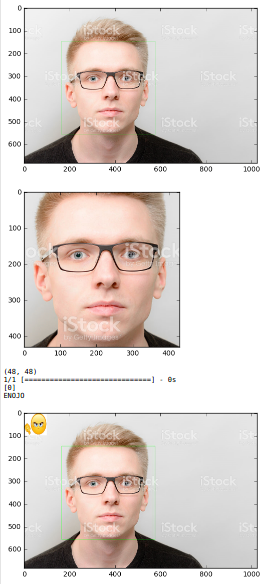
\includegraphics[angle=0,width=55mm]{Imagenes/test9.png}
           \caption{Test 9}
           \label{fig:test9} 
           
    \end{multicols}
        
\end{figure}
\end{frame}


